\chapter{Background}

Lorem ipsum dolor sit amet, consectetur adipiscing elit. In non molestie odio. Pellentesque volutpat, sem a viverra dictum, leo est scelerisque risus, ut convallis dui nulla a lacus. Proin mi magna, pharetra non ante sit amet, euismod lobortis odio. Donec gravida eu elit quis sagittis. Duis consequat, elit in fermentum rutrum, tellus dolor sodales ante, ac aliquam libero purus eu nisi. In aliquam nibh maximus varius blandit. Sed consequat libero faucibus vehicula gravida. Suspendisse vitae nisi ex. Quisque gravida risus ac dapibus blandit. Vestibulum mollis sollicitudin justo. Donec vel ipsum non ligula efficitur consequat. Morbi vulputate feugiat diam, rhoncus vehicula eros posuere vitae. Pellentesque sed egestas metus. Vestibulum libero elit, euismod quis vestibulum nec, vulputate at risus. In accumsan sem eu porta ultrices. Quisque sagittis massa felis, eget varius metus semper id. Vivamus tincidunt ipsum sem, sit amet eleifend diam tempor nec. Vivamus elementum, diam id lobortis mattis, nisi lacus. 

\section{Section title}
Lorem ipsum dolor sit amet, consectetur adipiscing elit. In non molestie odio. Pellentesque volutpat, sem a viverra dictum, leo est scelerisque risus, ut convallis dui nulla a lacus.  Proin mi magna, pharetra non ante sit amet, euismod lobortis odio. Donec gravida eu elit quis sagittis. Duis consequat, elit in fermentum rutrum, tellus dolor sodales ante, ac aliquam libero purus eu nisi. 

\section{Section title}
Lorem ipsum dolor sit amet, consectetur adipiscing elit. In non molestie odio. Pellentesque volutpat, sem a viverra dictum, leo est scelerisque risus, ut convallis dui nulla a lacus. Proin mi magna, pharetra non ante sit amet, euismod lobortis odio. Donec gravida eu elit quis sagittis. Duis consequat, elit in fermentum rutrum, tellus dolor sodales ante, ac aliquam libero purus eu nisi. 


\begin{lstlisting}[caption = Python Code Example]
def hello_world():
    @This part will be highlighted in red@
    print("Hello, world!")
hello_world()
\end{lstlisting}

\section{Section title}
Lorem ipsum dolor sit amet, consectetur adipiscing elit. In non molestie odio. Pellentesque volutpat, sem a viverra dictum, leo est scelerisque risus, ut convallis dui nulla a lacus. Proin mi magna, pharetra non ante sit amet, euismod lobortis odio. Duis consequat, elit in fermentum rutrum, tellus dolor sodales ante, ac aliquam libero purus eu nisi. 

\subsection{Sub-section title}
Lorem ipsum dolor sit amet, consectetur adipiscing elit. In non molestie odio. Pellentesque volutpat, sem a viverra dictum, leo est scelerisque risus, ut convallis dui nulla a lacus. Proin mi magna, pharetra non ante sit amet, euismod lobortis odio.  Donec gravida eu elit quis sagittis. Duis consequat, elit in fermentum rutrum, tellus dolor sodales ante, ac aliquam libero purus eu nisi. 

\subsection{Sub-section title}
Lorem ipsum dolor sit amet, consectetur adipiscing elit. In non molestie odio. Pellentesque volutpat, sem a viverra dictum, leo est scelerisque risus, ut convallis dui nulla a lacus. Proin mi magna, pharetra non ante sit amet, euismod lobortis odio. Donec gravida eu elit quis sagittis. Duis consequat, elit in fermentum rutrum, tellus dolor sodales ante, ac aliquam libero purus eu nisi.  Figure \ref{fig:main_figure} consists of two sub figures: Figure \ref{fig:subfigure_a} and Figure \ref{fig:subfigure_b}.     

\begin{figure}[tbh]
\centering
\sidesubfloat[]{
\includegraphics[width=0.4\textwidth]{Figures/cos1.jpeg}\label{fig:subfigure_a}}
\hfill
\sidesubfloat[]{
\includegraphics[width=0.4\textwidth]{Figures/cos2.jpeg}\label{fig:subfigure_b}}
%\caption[short title for list of figures]{long title for text}
\caption[The short caption of the figure with sub-figures goes here.]{The full caption of the figure with sub-figures goes here. \textit{(A)} Please describe the figure and figure legends for sub-figure A here. Lorem ipsum dolor sit amet, consectetur adipiscing elit. Etiam viverra. \textit{(B)} Please describe the figure and figure legends for sub-figure B here. Lorem ipsum dolor sit amet, consectetur adipiscing elit. Etiam viverra.}
\label{fig:main_figure}
\end{figure}

Lorem ipsum dolor sit amet, consectetur adipiscing elit. In non molestie odio. Pellentesque volutpat, sem a viverra dictum, leo est scelerisque risus, ut convallis dui nulla a lacus. Proin mi magna, pharetra non ante sit amet, euismod lobortis odio. Donec gravida eu elit quis sagittis. Duis consequat, elit in fermentum rutrum, tellus dolor sodales ante, ac aliquam libero purus eu nisi. Lorem ipsum dolor sit amet, consectetur adipiscing elit. In non molestie odio. Pellentesque volutpat, sem a viverra dictum, leo est scelerisque risus, ut convallis dui nulla a lacus. Proin mi magna, pharetra non ante sit amet, euismod lobortis odio. Donec gravida eu elit quis sagittis. Duis consequat, elit in fermentum rutrum, tellus dolor sodales ante, ac aliquam libero purus eu nisi. Lorem ipsum dolor sit amet, consectetur adipiscing elit. Duis consequat, elit in fermentum rutrum, tellus dolor sodales ante, ac aliquam libero purus eu nisi. Lorem ipsum dolor sit amet. Equation \ref{eq:1} exemplifies a standard power series, demonstrating how to include equations in your document.

\begin{equation} \label{eq:1}
\sum_{i=0}^{\infty} a_i x^i
\end{equation}


\section{Section Title}
In aliquam nibh maximus varius blandit. Sed consequat libero faucibus vehicula gravida. Suspendisse vitae nisi ex. Quisque gravida risus ac dapibus blandit. Vestibulum mollis sollicitudin justo. Donec vel ipsum non ligula efficitur consequat. Morbi vulputate feugiat diam, rhoncus vehicula eros posuere vitae. Pellentesque sed egestas metus. Vestibulum libero elit, euismod quis vestibulum nec, vulputate at risus. In accumsan sem eu porta ultrices. Quisque sagittis massa felis, eget varius metus semper id. Vivamus tincidunt ipsum sem, sit amet eleifend diam tempor nec. Vivamus elementum, diam id lobortis mattis, nisi lacus. Vivamus elementum, diam id lobortis mattis, nisi lacus. Vivamus elementum, diam id lobortis mattis, nisi lacus. Vivamus elementum, diam id lobortis mattis, nisi lacus.  Vivamus elementum, diam id lobortis mattis. 

Figure \ref{fig:logo_landscape} illustrates the process of incorporating figure in landscape orientation into your document. A similar approach can be employed for tables as well.

\begin{sidewaysfigure}[htbp]
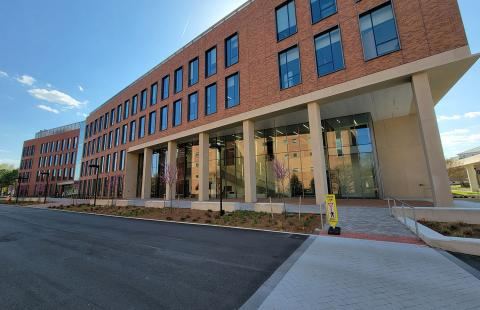
\includegraphics[width=\columnwidth]{Figures/cos_landscape.jpg}
\caption[The short figure caption goes here.]{The full figure caption goes here. Please describe the figure and figure legends here.}
\label{fig:logo_landscape}
\end{sidewaysfigure}

